\clearpage
\section{Visualising the hidden layer}

L'objectif dans cette section est de visualiser les représentations capturées par les unités cachées.
On voit que l'image génerée disposes de 25 images ressemblant aux chiffres et donc à des détecteurs qui 
recherchent des traits et d'autres motifs dans l'entrée.

\begin{figure}[!h]
    \begin{center}
        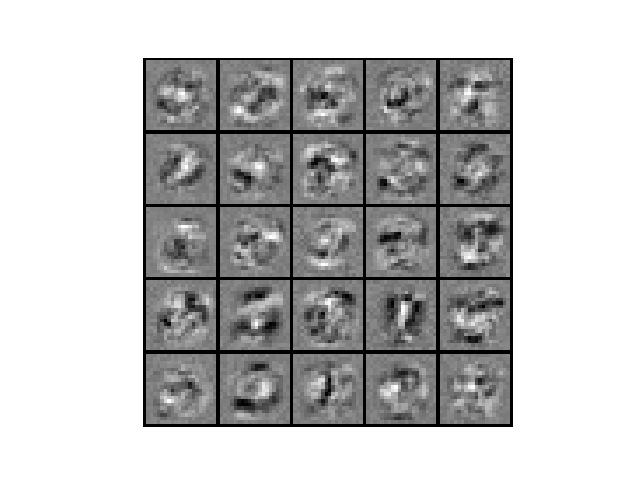
\includegraphics[width=0.75\textwidth]{./img/last.png}
        \caption{\label{fig:last}Visualization of Hidden Units}  
    \end{center}
\end{figure}

\section{Final analysis}

Dans cette section, l'objectif est d'augmenter la valeur de \textit{lambda} et de \textit{MaxIter} pour
essayer différentes configurations d'apprentissage du réseau neuronal et d'en évaluer la différence de 
performance. \\

Malheureusement pour cette partie, nos ordinateurs portable n'ont pas la capacité d'effectuer les calculs 
lorsque l'on incrémente MaxIter. On restera donc avec les résultats calculés préalablement.